\documentclass{csbulletin}
\selectlanguage{czech}
\usepackage[utf8]{inputenc}
\usepackage[all]{nowidow}
\usepackage{csquotes}
\usepackage[
  backend=biber,
  style=iso-numeric,
  sortlocale=cs,
  autolang=other,
  bibencoding=UTF8,
  mincitenames=2,
  maxcitenames=2,
]{biblatex}
\addbibresource{example.bib}
\usepackage{blindtext}
\usepackage[implicit=false,hidelinks]{hyperref}

% Pomocná makra
\def\TUG{TUG}
\def\TUGboat{TUGboat}
\let\stress\emph
\let\makro\texttt

\begin{document}
\hyphenation{Cross-Ref}
\title{Úvodník}
\EnglishTitle{Introductory Word}
\author{Petr Sojka}
\podpis{Masarykova univerzita, Fakulta informatiky, Botanická~68a, 602\,00 Brno\\
        \url{sojka@fi.muni.cz}}
\maketitle %[12dd]

Milé čtenářky a~čtenáři, \TeX istky a \TeX isté!

Je mi potěšením vám představit články tohoto čísla a seznámit vás 
s~informacemi ze světa našeho oblíbeného sázecího systému.
\smallskip

\noindent
\makeatletter
\ifcsbul@web
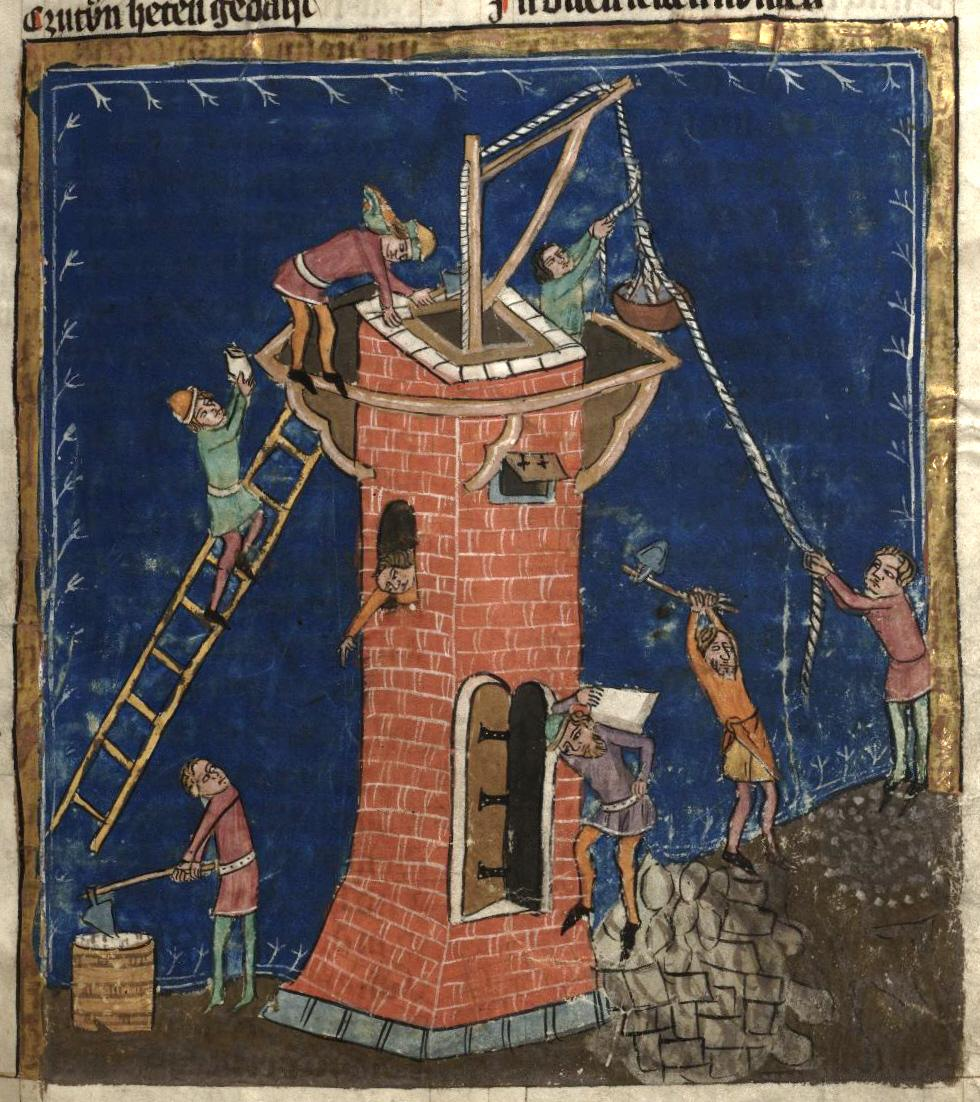
\includegraphics[width=.6\textwidth]{Weltchronik_Fulda_Aa88_016r_detail-web}\hfill
\else
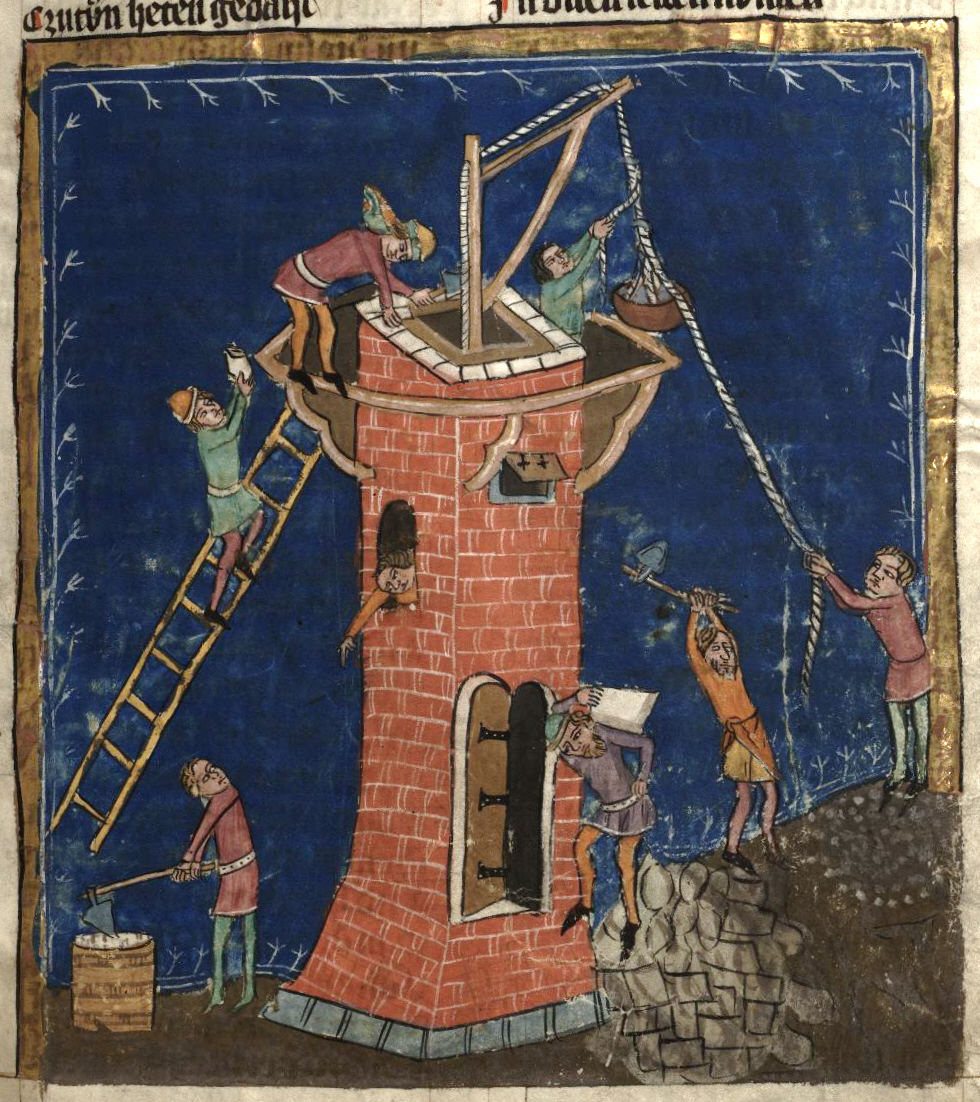
\includegraphics[width=.6\textwidth]{Weltchronik_Fulda_Aa88_016r_detail}\hfill
\fi
\makeatother
\begin{minipage}[b]{.37\textwidth}
Stavba babylonské věže ve Světové kronice Rudolfa von Ems, Praha, 3.~čtvrtina 14.~století.
\medskip

Autor: Anonymní (Meister~1) -- Hochschul- und Landes\-bibliothek Fulda
%, Volné dílo, https://commons.wikimedia.org/w/index.php?curid=23797681
\end{minipage}
\smallskip

Babylónské zmatení jazyků.
Tak nám připadá komunikace v~dnešním informačním věku.
Dávat věcem ta správná jména, odpovídající sémantice, a konzistentně je používat, to je, oč tu běží!

A běží o to v článku Vítka Starého Novotného, jehož nápad na nápadovník a~jeho realizace je tématem hlavního, prvního článku čísla. Láká Dášenka, Maxipes Fík a Pes Filipes, častá jména z článku a z titulní stránky tohoto čísla.
Pokud se ne\-necháte odradit asi deseti programovacími a značkovacími jazyky, které v~článku Vítek používá, dozvíte se základní principy jazykových modelů a také způsob, jakým je využijete přímo při tvůrčím psaní.
Pojďte zjistit, k čemu jsou dobré náhodné procházky, programovací jazyk expl3, Katzův couvající jazykový model, zapomnětlivost, náhodná semínka či multi\-plikativní lineární kongruenční generátor.  
Dostanete \uv{na konečky svých prstů} a do svého dokumentu informace hlubokých jazykových modelů, což dá vašim textům patřičnou hloubku nebo výšku srovnatelnou s babylónskou věží nebo odbřemení od explicitního přepínání jazyků tím, že \uv{umělá inteligence} dobře odhadne použitý jazyk textu.
Jestli chcete jít s dobou, tak do toho!

Sazba hudebních skladeb je vzhledem ke složitosti notového zápisu výzvou. Možnostem sazby not nejen MusiX\TeX em, ale využití specializovaných preprocesorů, které přípravu notového zápisu usnadní, se věnuje přehledový článeček Karla Šebely.

Matúš Vančík se dělí o to, co ho zaujalo v prezentacích hlavní \TeX ovské konference TUG 2022.
Způsob, jak vznikají makrobalíčky, jak je kombinovat nebo jak realizovat puzzle s~logem Fakulty informatiky Masarykovy univerzity, jsou jen některé z nových informací, kterými vás článek po přečtení obohatí.

Číslo uzavírá již \emph{třinácté} pokračování komentovaných ukázek \TeX ových maker z pera Petera Wilsona, které pro čtenáře Zpravodaje již třináct let\footnote{K 
%\href{https://dml.cz/advanced-search?num_search_field=3&results_per_page=30&scope=10338.dmlcz%2F148724&field1=title&query1=&conjunction2=AND&field2=author&query2=Peter+Wilson&conjunction3=AND&field3=msc&query3=&submit=Go}%
{celému seriálu překladů Glisterings} se můžete vrátit na stránkách \href{https://dml.cz}{DML.CZ}, kde péčí aktivních členů sdružení~\cite{tex:vrabcova2022,tex:NovotnyVH2021} vznikl archiv celého Zpravodaje~\cite{tex:Zpravodaj}.} překládá ze série Glisterings z~časopisu \TUGboat\ náš pan šéfredaktor Honza Šustek.

\medskip
Závěrem chci poděkovat aktivním \TeX istům, autorům, členům sdružení
uživatelů \TeX u.
Bez nich, převážně členů \CSTUG u a \TUG u a jejich \uv{labour of love} by to nebylo možné.

\printbibliography
 
\begin{summary}
Go forth and participate in \CSTUG\ to make the bright future of \TeX\,\&\,Friends a~reality!
\emph{You can!}
\end{summary}
\end{document}
